% main.tex

%specify class of document
\documentclass[11pt, a4paper]{article}

%specify packages used 
\usepackage{microtype}		       		%use package for minor typographical adjustments
\usepackage{graphicx} 		       		%use package for diagram 
\usepackage{listings}                  		%use package for c++ code in appendix
\usepackage{color}                     		%use package for code listings
\usepackage[utf8]{inputenc}            		%use package for colours in code
\usepackage{amsmath}                   		%use package for various math symbols
\usepackage{amsfonts}                  		%use package for number sets
\usepackage{bm}			       		%use package for bolds in math mode
\usepackage{hyperref}                  		%use package for hyperlinks
\usepackage{algpseudocode}             		%use package for pseudocode
\usepackage{algorithm}                 		%use package for pseudocode
\usepackage{fullpage}                  		%use package for full page size
\usepackage{tikz}		       		%use package for diagram drawings
\usepackage[justification=centering]{caption}   %use package for multiple figures
\usepackage{subcaption}                		%use package for multiple figures
\usepackage{tabularx}		      		%use package for tables
\usepackage{array}                     		%use package for centering table contents
%\usepackage{url}                       	 %use package to display urls properly

%set graphics path
\graphicspath{{images/}}

%define colours for code listings
\definecolor{codegreen}{rgb}{0,0.6,0}
\definecolor{codegray}{rgb}{0.5,0.5,0.5}
\definecolor{codepurple}{rgb}{0.58,0,0.82}
\definecolor{backcolour}{rgb}{0.95,0.95,0.92}

%define a style for the listings
\lstdefinestyle{mystyle}{
    backgroundcolor=\color{backcolour},
    commentstyle=\color{codegreen},
    keywordstyle=\color{magenta},
    numberstyle=\tiny\color{codegray},
    stringstyle=\color{codepurple},
    basicstyle=\footnotesize,
    breakatwhitespace=false,
    breaklines=true,
    captionpos=b,
    keepspaces=true,
    numbers=left,
    numbersep=5pt,
    showspaces=false,
    showstringspaces=false,
    showtabs=false,
    tabsize=2,
    language=C++
}

%set style of listing to that defined above
\lstset{style=mystyle}

%use tikz library for shapes
\usetikzlibrary{shapes.geometric, arrows}

%define block styles in tikz
\tikzstyle{startstop} = [rectangle, rounded corners, minimum width=3cm, minimum height=1cm, text centered, draw=black, fill=red!30]
\tikzstyle{io} = [trapezium, trapezium left angle=70, trapezium right angle=110, minimum width=3cm, minimum height=1cm, text centered, draw=black, fill=blue!30]
\tikzstyle{process} = [rectangle, minimum width=3cm, minimum height=1cm, text centered, draw=black, fill=orange!30]
\tikzstyle{decision} = [diamond, minimum width=3cm, minimum height=1cm, text centered, draw=black, fill=green!30]
\tikzstyle{arrow} = [thick,->,>=stealth]

%set style of bibliography
\bibliographystyle{unsrt}

%set style of footnotes
\renewcommand{\thefootnote}{\roman{footnote}}

%define command shortcuts
\newcommand{\be}{\begin{equation}}
\newcommand{\ee}{\end{equation}}

%redefine columns for tabularx
\newcolumntype{Y}{>{\centering \arraybackslash}X}

\begin{document}

\title{On numerical approximations to solutions of Laplace's equation for different
electrostatic configurations}
\author{S. Brown, F. Hayes, L. Heikkil{\"a}, D. Richardson,\\
	School of Physics and Astronomy,\\
	University of Glasgow,\\
	Glasgow, United Kingdom}
\date{\today}
\maketitle

\begin{abstract}

The behaviour of the electric field under the presence and influence of solid
conducting objects is modelled and studied. Finite difference methods, namely
relaxation methods, are employed to solve the Laplace equation numerically,
to find the approximate form of the electrostatic potential, and hence the electric
field, present in various electrostatic systems.

We explicitly focus on two such systems: first, the case of a long perfectly conducting
cylinder centred between two infinite planes at potential $+V$ and $-V$; and secondly 
the case of a silicon detector---a system composed of two silicon wafers with segmented
doped implants at ground potential on one side and a uniform doped implant on the
other side, held at a potential $+V$. We present the analytical solution of the first
system. This solution is then compared to the approximate numerical solution produced
by five different relaxation methods, and examine the relative error and relative
convergence of each of them. We then conclude that the method of 
\emph{Checkerboard Updating with successive over-relaxation} is best.

The design, implementation and operation of a software package we have
developed, named \lstinline|eStatics|---which is capable of solving
Laplace's equation for arbitrary constant boundary conditions---is discussed.
Output of the package is presented for different electrostatic systems, and
opportunities for further work are proposed.

\end{abstract}

% DO NOT INCLUDE IN FINAL VERSION
%%%%%%%%%%%%%%%%%%%%%%%%%%%%%%%%
\newpage                       %
\tableofcontents               %
\newpage                       %
%%%%%%%%%%%%%%%%%%%%%%%%%%%%%%%%

\section{Introduction}
\subsection{Laplace's Equation}

The Laplace equation is a linear second-order partial differential equation that can be
used to describe steady-state distributions of heat, fluids and potential where there
are no sources. It states that the divergence of the gradient of a function, $\phi$ say,
is zero. Symbolically:
%
\be
\nabla ^2 \phi = 0
\ee
%
where $\nabla^2$ is called the \emph{Laplacian operator}. The study of solutions to
this equation is known as \emph{potential theory}.

The exact form of the equation is dependent upon the co-ordinate system in which one
considers it. In two dimensions, where subscripts denote partial differentiation with
respect to that variable:

\begin{center}
\begin{tabularx}{0.6\textwidth}{|Y|Y|}
\hline
\emph{Cartesian co-ordinates} & \emph{Polar co-ordinates} \\
$\phi_{xx}+\phi_{yy}=0$ & $\phi_{rr}+\frac{1}{r}\phi_r+\frac{1}{r^2}\phi_{\theta \theta}=0$ \\
\hline
\end{tabularx}
\end{center}

The Laplace equation shall now be derived in the context of electromagnetism.

\subsubsection{Derivation of Laplace equation in Electomagentism}
Consider the two Maxwell equations~\cite{em} that describe the electric field,
\textbf{E}: Gauss' Law and Faraday's Law.

Gauss' Law may used to express the relation between the \emph{divergence} of the
electric field, and the \emph{charge density} $\rho$,
%
\be
\nabla \cdot \bm{E} = \frac{\rho}{\epsilon_0}
\ee
%
where $\epsilon_0$ is the \emph{permittivity of free space}. Alternatively (c.f.
\emph{the Divergence Theorem}), it can be expressed in its integral form, as:
%
\be
\oint \limits_S \bm{E} \cdot d\bm{A} = \frac{Q}{\epsilon_0}
\ee
%
where the integral is taken over a closed surface, $S$, and $Q$ is the enclosed charge.
In the absence of charge, as is the case in free space outside a conductor, this
reduces to the statement that the electric field is \emph{solenoidal}
($\nabla \cdot \bm{E}=0$).

The Maxwell-Faraday equation expresses the relation between the \emph{curl} of the
electric field and the time derivative of the magnetic field, denoted \textbf{B}:
%
\be
\nabla \times \bm{E} = - \frac{\partial \bm{B}}{\partial t}
\ee

If the magnetic field is constant, this equation reduces to the statement that
the electric field is \emph{irrotational} ($\nabla \times \bm{E}=0$). A
consequence of irrotationality is that the electric field may then be written as
the gradient of some scalar potential, $\phi$ say. Mathematically:
%
\be
\bm{E} = -\nabla \phi
\ee
%
where the negative sign is convention. This scalar potential is called the
\emph{electrostatic potential}. This results in \emph{Laplace's equation}:
%
\be
\nabla^2 \phi = 0
\ee

This is a linear second-order partial differential equation that can be solved, given
some well-posed boundary conditions, to find the electrostatic potential and hence
electric field for some physical system. This, in turn, can be used to find the
equations of motion of test particles within the system, via the Lorentz force law.

The following analysis occurs in the context of electromagnetism, where the equation
describes the electrostatic potential in a a charge-free region, but can be easily
generalised to other areas of physics were the Laplace equation occurs, for example,
fluid dynamics, where it describes the flow of an incompressible fluid with no sources
or sinks; to astronomy, where it describes the gravitational potential in a region
containing no matter. See pp.679 of~\cite{mm}.

\subsection{Description of Physical Systems}

Consider a perfectly uniform electric field between two infinite planes at potentials
$V$ and $-V$, a distance $2d$ apart, with an infinitely long perfectly conducting
cylinder, of radius $R$, placed into the centre of the field, at ground potential,
as in Figure~\ref{fig:sys one}. The resulting form of the electrostatic potential,
and hence the electric field, surrounding the cylinder, can be analytically deduced.

\begin{figure}[h!]
\begin{center}
\begin{tikzpicture}
\draw (0,0) node[below] {$x = -d$} -- (0,4.8) node[above] {$\phi = V$}; 
\draw (8,0) node[below] {$x = d$} -- (8,4.8) node[above] {$\phi = -V$}; 
\draw (4,2.4) circle (1cm) node[below] {$\phi=0$};
\draw[dashed] (4,2.4) -- (4.6,3.2) node[pos=0.5,above left] {$R$};
\end{tikzpicture}
\end{center}
\caption{Cross-sectional diagram of System One}
\label{fig:sys one}
\end{figure}

The second system considered was a silicon detector---a system consisting of two
silicon wafers, one segmented with doped implants at ground potential and the other,
referred to as the backplane, uniformly doped, held at a potential $+V$, as shown
in Figure~\ref{fig:sys two}. 

\begin{figure}[h!]
\begin{center}
\begin{tikzpicture}
\draw (0,0) -- (9.6,0) node[right] {$\phi = V$}; 
\draw (0,4) -- (9.6,4) node[pos=0.25, above, font=\footnotesize] {GND} node[pos=0.5, above, font=\footnotesize] {GND} node[pos=0.75,above, font=\footnotesize] {GND}; 
\draw (2,4) rectangle (2.8,3.8);
\draw (4.4,4) rectangle (5.2,3.8);
\draw (6.8,4) rectangle (7.6,3.8);
\end{tikzpicture}
\end{center}
\caption{Cross-sectional diagram of System Two}
\label{fig:sys two}
\end{figure}

System One can be solved analytically, as will be shown in the subsequent section. This
solution shall be used to compare the accuracy of different numerical methods in solving
System One, and to decide which method is best suited to solve more complex systems, such
as System Two, that do not have analytical solutions.

\subsection{Analytical Solution of System One}

First, the three-dimensional problem can be reduced entirely to two
dimensions due to the translation symmetry of the system along the length of the
cylinder. So, consider a cross-section of the system and introduce a polar
co-ordinate system, with origin centred on the centre of the cylinder, as this permits
one to exploit the rotational symmetry of the system.

Laplace's equation in plane polar co-ordinates is: 
%
\be
\frac{\partial^2 \phi}{\partial r^2}+\frac{1}{r}\frac{\partial \phi}{\partial r}+\frac{1}{r^2}\frac{\partial^2 \phi}{\partial \theta^2}
= \frac{1}{r}\frac{\partial}{\partial r}(r \frac{\partial \phi}{\partial r}) + \frac{1}{r^2}\frac{\partial ^2 \phi}{\partial \theta^2}
= 0
\ee

Propose a separable solution of the form $\phi = f(r)g(\theta)$ for two unknown
functions $f$ and $g$. Upon substitution:
%
\be
\frac{r}{f(r)}\frac{d}{dr}(r \frac{df(r)}{dr}) =- \frac{1}{g(\theta)}\frac{d^2 g(\theta)}{d\theta^2}
\ee

Since the left-hand side is solely a function of $r$---and the right-hand side of
$\theta$---they both must be constant if the relation is to hold for arbitrary values
of $r$ and $\theta$. Then set this constant equal to $k^2$, for some constant
$k\in\mathbb{R}$. This gives two second-order ordinary differential equations:
%
\be
r\frac{d}{dr}(r \frac{df(r)}{dr}) = k^2 f(r) \qquad
\frac{d^2 g(\theta)}{d\theta^2}=-k^2 g(\theta)
\ee

For the case $k=0$, these equations have solutions
$f(r)=\alpha \ln(r) + \beta$ and $g(\theta) = \gamma \theta + \delta$.
For non-zero $k$, they have solutions
%
\be
f(r)=\alpha_k r^k + \beta_k r^{-k}
\qquad
g(\theta)= \gamma_k \sin(k\theta)+\delta_k \cos(k\theta)
\ee

For consistency, $g$ is expected to be single-valued and periodic, namely that
$g(\theta)=g(\theta + 2\pi)$, so that $k$ can only take integer values. Hence, by
the principle of superposition, the general solution of Laplace's equation in polar
co-ordinates is a sum of such terms:
%
\be
\phi(r,\theta)
= f(r)g(\theta)
= (\alpha \ln(r) + \beta)(\gamma\theta + \delta) + \sum_{n=1}^{\infty}(\alpha_n r^n+\beta_n r^{-n})(\gamma_n \sin(n\theta) + \delta_n \cos(n\theta))
\ee
%
where negative values of $n$ are omitted as they are included in the terms for positive
$n$. See pp. 725-727 of~\cite{mm}. 

For a particular solution to the system considered here boundary conditions must be
imposed. Specifically, \emph{Dirichlet boundary conditions} are used, where the value
of the solution at each boundary is specified.

By considering the geometry of the system, a solution that is symmetric about $\theta=0$
is expected. This directly implies that $\gamma = 0$ and $\gamma_n=0$, $\forall n$
as $\sin(\theta)$ and $\theta$ are both anti-symmetric (or odd) about the origin.
Additionally, the potential is finite as $r \rightarrow \infty$, which implies that
$\alpha$ and $\alpha_n$ are both zero. This gives:
%
\be
\phi(r,\theta)=\beta + \sum_{n=1}^{\infty}(\frac{\beta_n}{r^n} \cos(n\theta))
\ee
%
where the $\beta$'s have absorbed other constants. In particular, as
$r \rightarrow \infty$, that is as the influence of the cylinder becomes negligible,
the potential is expected to be linearly decreasing between the plates. Hence,
mathematically, $\phi=-\frac{V}{d}x=-\frac{V}{d}r\cos(\theta)$ in polar co-ordinates.
Since the infinite sum vanishes at infinity, $\beta=-\frac{V}{d}r\cos(\theta)$.

Thus
%
\be
\phi(r,\theta)=-\frac{V}{d}r\cos(\theta) + \sum_{n=1}^{\infty}(\frac{\beta_n}{r^n} \cos(n\theta))
              =(\frac{\beta_1}{r}-\frac{V}{d}r)\cos(\theta) + \sum_{n=2}^{\infty}(\frac{\beta_n}{r^n} \cos(n\theta))
\ee

The potential is expected to be continuous at the surface of the cylinder:
$\phi(r=R,\theta)=0$, so that $\beta_1=\frac{VR^2}{d}$ and $\beta_{n \geq 2}=0$,
since the set $\{\cos(n\theta)\}$ are linearly independent functions.

Thus, the final form for the electrostatic potential for System One (see
Figure~\ref{fig:analytic}) is
%
\be
\phi(r,\theta)=
\begin{cases} \quad \qquad 0, & \quad r \leq a \\
\frac{V}{d}(\frac{R^2}{r}-r)\cos(\theta), & \quad r > a
\end{cases}
\ee

\begin{figure}
\begin{center}
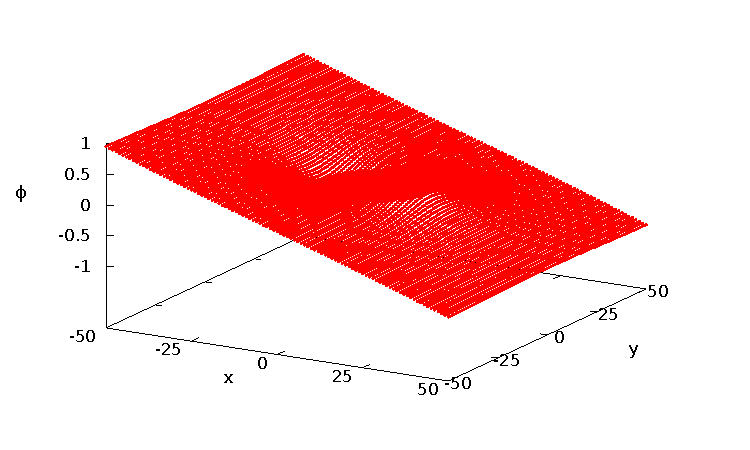
\includegraphics{analytic.pdf}
\caption{Analytical solution for the electrostatic potential of System One, with $V=1$,
$R=15$, $d=50$}
\label{fig:analytic}
\end{center}
\end{figure}

\section{Numerical Methods}
\subsection{Finite Difference Methods}

System One is a very idealised system that is not practically reasonable, for example
charged planes that are infinite in extent do not exist. For real-world systems
it is difficult, and often impossible, to express boundary conditions in a manner that
is algebraically utilisable and is thus impossible to find a particular analytical
solution to Laplace's equation for arbitrary, non-trivial, boundary conditions. Solutions
for these types of systems must be numerically approximated.

To numerically approximate the solution to a differential equation it is
necessary to approximate the derivative of a function. The usual method employed to
do this is finite differencing. This approximates the derivative by using explicit
differencing to step the function from one value to the next in small 
increments of some variable. The smaller the increment used, the more accurate
the approximation, but the longer and more computationally intensive the process.

To approximate the first derivative of a function $f(t)$, say, with respect to the
variable $t$. The simplest way to do this is to discretise the definition of the
derivative and write
%
\be
\frac{df}{dt} = \lim_{\Delta t \to 0} \frac{f(t+\Delta t) - f(t)}{\Delta t} \approx \frac{f(t+\Delta t) - f(t)}{\Delta t}
\ee
%
where $f(t+\Delta t)$ and $f(t)$ are two values of $f$, evaluated at two points
a distance $\Delta t$ apart, and $\Delta t$ is assumed to be small enough that
the approximation is good. This is known as the \emph{forward difference approximation}
and has a truncation error $\sim \frac{\Delta t}{2}$.
Alternatively, one can employ the \emph{central difference approximation}:
$\frac{df}{dt}\approx \frac{f(t+\Delta t) - f(t-\Delta t)}{2 \Delta t}$, which has
truncation error $\sim \frac{\Delta t^2}{6}$.

Similarly, to approximate the second derivative of a function:
%
\be
\frac{d^2 f}{dt^2} \approx \frac{f'(t) - f'(t-h)}{\Delta t} \\
= \frac{\frac{f(t +\Delta t) - f(t)}{\Delta t} - \frac{f(t) - f(t -\Delta t)}{\Delta t}}{\Delta t} \\
= \frac{f(t +\Delta t) - 2f(t) + f(t-\Delta t)}{\Delta t ^2}
\ee
%
This has truncation error $\sim \frac{\Delta t^2}{2}$. See pp. 1019 of~\cite{mm} for a
fuller discussion.

\subsection{Discretisation of Laplace's Equation}

To numerically solve the Laplace equation it must be expressed in a discrete form.
Define a rectangular region, of dimension $a\times b$, on which to discretise
Laplace's equation, given by:
%
\be
\{(x,y)|\:0<x<a, 0<y<b\}
\ee
%
and create a grid of points at which to evaluate the potential of spacial separation
$\Delta x$ in the $x$ direction, and $\Delta y$ in the $y$ direction. The grid is
compose of interior points that change value; and exterior points on which constant
Dirichlet boundary conditions are imposed.

For simplicity, the Laplace equation in two-dimensional Cartesian co-ordinates is
discretised:
% 
\be 
\frac{\partial^2 \phi}{\partial x^2}+\frac{\partial^2 \phi}{\partial y^2} = 0
\label{eq:laplace}
\ee 

Writing the value of the potential at position $(x_j,y_k)$ on the grid as $\phi_{j,k}$,
Eqn.~\ref{eq:laplace} can be discretised as:
% 
\be
\frac{\phi_{j+1,k}-2\phi_{j,k}+\phi_{j-1,k}}{\Delta x^2} = - \frac{\phi_{j,k+1}-2\phi_{j,k}+\phi_{j,k-1}}{\Delta y^2}
\ee
%
where $j$ and $k$ index the $x$ and $y$ directions respectively. See pp. 1031
of~\cite{mm}.

For a unique spacing $\Delta=\Delta x=\Delta y$ this reduces to the statement that
the value of the potential at a specific point is the average of the value of the
potential at the four surrounding points: 
%
\be
\phi_{j,k}= \frac{1}{4}(\phi_{j-1,k}+\phi_{j+1,k}+\phi_{j,k-1}+\phi_{j,k+1})
\label{eq:relax}
\ee

\subsection{Jacobi's Iterative Method}

Using some initial guess for the value of the potential at all points on the
grid, $\phi_{j,k,0}$, say, Eqn~\ref{eq:relax} can be evaluated simultaneously at all
points on the grid to generate a new better approximation for the potential,
$\phi_{j,k,1}$. Iterating this process $n$ times gives:
%
\be
\phi_{j,k,n+1}= \frac{1}{4}(\phi_{j-1,k,n}+\phi_{j+1,k,n}+\phi_{j,k-1,n}+\phi_{j,k+1,n})
\ee
%
This is known as \emph{Jacobi's iterative method}, the simplest version of a
\emph{relaxation method}, an algorithm where the numerical approximation converges or
\emph{relaxes} towards the analytical solution with increasing iterations. 

\subsection{The Gauss-Seidel Method}

As the grid is iterated through and relaxation is applied, points at which the potential
has already been updated---namely $\phi_{j-1,k}$ and $\phi_{j,k-1}$---are presumably
more accurate to the correct solution than points that have not been updated.
An alternative relaxation method, known as the \emph{Gauss-Seidel method}, takes use of
this supposition and defines an iterative scheme given by:
%
\be
\phi_{j,k,n+1}= \frac{1}{4}(\phi_{j-1,k,n+1}+\phi_{j+1,k,n}+\phi_{j,k-1,n+1}+\phi_{j,k+1,n})
\ee

It can be shown that this method converges faster than Jacobi's iterative
method, and it also has the advantage of not requiring the previous value of the 
potential at each grid point to be stored, thus reducing computation time.

\subsection{Successive Over-Relaxation}
Like the Gauss-Seidel method, the successive over-relaxation method uses two
points from the previous iteration and the two updated points. It also
utilises the point $\phi_{i,j,n-1}$, and applies over-relaxation by using a
constant $s$ known as the relaxation parameter.
%
\be
\phi_{j,k,n+1}=(1-s)\phi_{j,k,n}+\frac{s}{4}(\phi_{j-1,k,n+1}+\phi_{j+1,k,n}+\phi_{j,k-1,n+1}+\phi_{j,k+1,n})
\ee

The optimum value for the relaxation parameter cannot be easily determined
arithmetically but to allow the system to converge, the value is always
within $s\in[1,2]$. The optimal value for a square grid (see~\cite{sor})
can be approximated using:
%
\be
 s_{opt} = \frac{2}{1+\sin(\frac{\pi}{n})} \approx \frac{2}{1+\frac{\pi}{n}}
\ee
%
for an $n \times n$ square grid.

The method reduces iterations by a considerable amount depending on the value
of the relaxation parameter used.


\subsection{Checkerboard (Red-Black) Updating}

In each of the previous methods, the value of the potential is calculated from, at most,
its previous value at the current point and the current or previous values of the
potential at the four neighbouring points. Noting this, let $\phi_{j,k}$ be denoted as
\emph{odd} if $j+k$ is odd, and even otherwise. Then the potential at each even point
solely depends on the potential at odd points, and vice-versa. In principle, then,
the grid of points at which the potential is approximated could be iterated through,
and all the odd points updated, and then re-iterated through, updating all the
even points using the value of the potential at the newly updated odd points. Such an
iterative scheme exists, and is known as \emph{Checkerboard (Red-Black) Updating}~\cite{wallach}. The
method essentially reduces a system of $N$ linear equations into two coupled systems
of $\frac{N}{2}$ linear equations that can be solved separately.

The method can be shown to be a more convergent method than those outlined previously,
and successive over-relaxation can easily be implemented within the scheme.
Figure~\ref{fig:checker} shows an illustration of the algorithm.

\begin{figure}[h!]
\begin{center}
	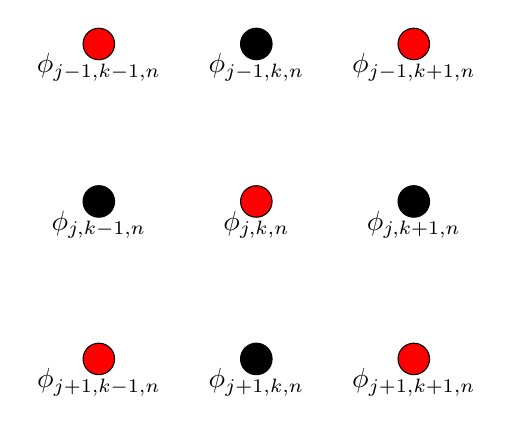
\begin{tikzpicture}
	\draw[fill=red] (0,0) circle (0.2cm) node[below] {$\phi_{j+1,k-1,n}$}; 
	\draw[fill=black] (2,0) circle (0.2cm) node[below] {$\phi_{j+1,k,n}$}; 
	\draw[fill=red] (4,0) circle (0.2cm) node[below] {$\phi_{j+1,k+1,n}$};
	\draw[fill=black] (0,2) circle (0.2cm) node[below] {$\phi_{j,k-1,n}$};
	\draw[fill=red] (2,2) circle (0.2cm) node[below] {$\phi_{j,k,n}$};
	\draw[fill=black] (4,2) circle (0.2cm) node[below] {$\phi_{j,k+1,n}$};
	\draw[fill=red] (0,4) circle (0.2cm) node[below] {$\phi_{j-1,k-1,n}$};
	\draw[fill=black] (2,4) circle (0.2cm) node[below] {$\phi_{j-1,k,n}$};
	\draw[fill=red] (4,4) circle (0.2cm) node[below] {$\phi_{j-1,k+1,n}$};
	\end{tikzpicture}
\end{center}
\caption{An illustration of checkerboard updating. The black points are updated first,
and then red points are updated using the newly updated black points.}
\label{fig:checker}
\end{figure}

Another advantage of this method is that due to the independent nature of the red and
black points, it lends itself particularly well to the introduction of parallel 
computing, which can reduce computation time even more, particularly for larger grid
sizes.

For a discussion of the implementation of these methods in C++, see~\cite{nr}.

\subsection{Comparison of methods}

To decide which relaxation method was best to implement in the software package,
each method was coded into C++ and ran to solve Laplace's equation for System One.
Each method works and the resulting numerical approximations can be seen in
Appendix~\ref{app:comparison}.

As there is very little graphical difference between each method, more quantitative
comparison methods were employed, namely the relative convergence and error---as
compared to the analytical solution---of each method, and their dependence on number
of iterations, was studied. The CPU time for each method was also studied. The results
are also summarised in Appendix~\ref{app:compare}.

The following conclusions were drawn from the data: the addition of successive
over-relaxation causes drastic increase in convergence; average relative error
essentially converges for all methods; and CPU time is not an important factor.

Hence, Checkerboard Updating with successive over-relaxation was chosen to be used
in the genereal software package, since it converges in the least iterations,
and hence least time, but to the same accuracy as the other methods.

\section{Software Package \emph{eStatics} for general electrostatic systems}

A general software package in C++ was developed to solve and plot the potential and
electric field for an arbitrary electrostatic system. It accepts input of a coloured
bitmap, where the colours represent different constant potentials, converts this into
an array of values and applies checkerboard updating with successive over-relaxation
to this array until each grid point is deemed to have converged. The package then
returns plots of the resultant electrostatic potential, equipotential lines and electric
field.

Appendix~\ref{app:flowchart} shows a flowchart of the software.

\subsection{Bitmaps}
Unlike PNG, GIF and JPEG image files, BMP files are uncompressed allowing them to be manipulated easily by programs. In a BMP file, there are three bytes of memory for each pixel to store a value for the colour scale for three different colours: blue, green and red. The colour scale runs from 0 to 255 (0 being no contribution from that colour to the pixels colour and 255 being maximum contribution) and allows the pixel to have a range of 16,777,216 individual variations in colour.

The potential boundaries for each system were drawn onto a blank BMP file where coloured areas are areas of constant potential and blank white pixels are areas of unsolved potential. Each colour has a different value of potential to assign to the points it covers. For the systems examined, only a minimum of four different potentials were needed and therefore were represented by the colours black, red, green and blue. The potential assigned to each colour was taken off the command line arguments. The strengths of green, blue and red can be determined comparing which colour scale is largest, and black is simply the absence of any values for the colour scales (BMP files of both the systems are found in the Appendix~\ref{app:bitmaps}).

eStatics analyses each pixels colour and maps boundary conditions onto arrays of the same dimensions as the pixel array, these arrays are: the potential grid stores the potential of the boundaries and the unsolved areas (initially set to zero) and the bool mask which stores boolean elements set to true at boundary locations and false at unsolved areas to keep boundaries constant. To extract the information from the BMP files, a library of commands called 'bitmap\textunderscore image.hpp'~\cite{arash} was used. This allowed the program to open the BMP file  by taking the file name from a command line argument before extracting the dimensions of the image and assigning the width and height to integers.

The pixel array is looped through and integers are assigned with the value of the colour scale. The colour of the pixel is determined by comparing the colour scales; if the red colour scale is greater than the blue and green colour scales, then the point on the potential grid is given the potential from the command line arguments assigned to red pixels and \emph{vice-versa} for green and blue. If the colour scales all equal zero, then the colour of the pixel is said to be black. The value on the potential grid with the same location as the pixel is assigned with the value of potential associated with the pixels colour. Points on the boolean array at the locations of coloured pixels is set to true.


\subsection{Data Handling}
		In order to simplify the passing of pertinent data to and from sub-functions, two structs were created. Structs --- or records --- are a type of data structure which can hold an arbitrary number of fields, each of which can be of a different data type. This makes them ideal for this case; arrays of type \lstinline|double| are required to hold the system to be solved and the gradient components of the electric field, \lstinline|int| variables can be used to hold the dimensions of the array --- which allows the solver to simply read this information rather than calculate it when needed - and to pass back the number of iterations required to meet the desired convergence, and the \lstinline|bool| data type can be used to write-protect boundary elements. This final point is discussed in detail in section~\ref{sec:mask}.
		
		In the case of \lstinline|eStatics|, a global pointer to the data struct was defined as \lstinline|extern| in the header file and created outside the main function. This allows the designation of a memory address to the structure which can be seen by all sub-routines, allowing each to read from and write to the fields contained within it. The \lstinline|new| command is used to dynamically assign memory to those fields, and expand them when needed. This allows systems of arbitrary size, or fineness of grid, to be solved by the software package. Another benefit of using a global struct is that variables such as system dimension, desired convergence, and maximum iterations need only be written once when building the system --- from then on only memory reads are required. Finally, RAM usage is lowered due the passing of only one set of data by address; this is due to there being no need to copy data and pass it by value to sub-routines.

\subsection{Element Protection}
\label{sec:mask}
		A problem with iterative algorithms such as the Finite Difference Method (FDM) is that the initial boundary conditions can be eroded by successive averaging. To counteract this, these boundaries must either be rewritten with each iteration --- with significant costs in terms of time due to extra read/write cycles being required, and RAM usage due to a copy of the initial grid having to be kept in memory --- or write-protected for the duration of the program. For the latter, which can avoid or reduce the noted costs of the former, the boolean data type is ideally suited.
		
		\subsubsection{Boolean Mask}
		
		Boolean is a data type with only two possible values; true or false. As such, each boolean --- or \lstinline|bool| --- requires very little memory. Typically, a boolean variable is the smallest possible variable in terms of RAM requirements. This makes them ideal for use in the write-protection of boundary elements, as it drastically lowers the overhead in this area. In order to utilise this, a boolean array of equal dimension to the system array is created whilst the user-provided bitmap image is being analysed. If an element, or pixel, of the system is defined as a boundary element the corresponding element in the boolean mask is set to true. All non-boundary elements are set to false.
		
		Next, whilst the solver is running through the system array point-by-point, it first checks the corresponding element in the mask. If this boolean is found to be true, the solver ignores that element. This saves time, as no further calculation needs to take place on that element.


\subsection{Convergence}
The successive over-relaxation method does not have an easily quantifiable error. The truncation error from the finite difference approximation is found by calculating higher derivatives than the solution requires and therefore requires substantially more computing to determine. Instead the precision of our results are analysed.
\\
The precision is related to how close a numerically determined value is from the true value it is converging to. If a numerical process determines a value $\tilde{x}$ on iteration $n$ which is converging to $x$, then:
\begin{align*}
\lim_{n \rightarrow \infty}\tilde{x} = x                     
\end{align*}
As the true value $x$ is constant, if the expression is differentiated with respect to the number of iterations, the rate of change of the determined value $\tilde{x}$ over iterations tends towards zero:
\begin{align*}
\lim_{n \rightarrow \infty}\frac{d\tilde{x}}{dn} = \lim_{n \rightarrow \infty} (\tilde{x}^{n} - \tilde{x}^{n-1}) = 0                     
\end{align*}
The magnitude of the difference of determined values $\tilde{x}$ between successive iterations is then related to how close the value is to the true value $x$. The closer the value is to zero, the more precise the value.
\subsection{Absolute Convergence}
The magnitude of the difference of the potential between successive iterations at some point is referred to as absolute convergence $\epsilon_{abs}$ of that point:
\begin{align*}
\epsilon_{abs \; i,j}^{n} = |\tilde{\phi}^{n} - \tilde{\phi}^{n-1}|
\end{align*}
This value is used in the program to limit the number of iterations the numerical process undertakes and also is used to 'lock' converged points to reduce calculations per iteration.
\subsection{Convergence Limit}
Within the program, the precision of the numerical solution is analysed as an indicator of accuracy. The absolute convergence is found for every point on the potential grid to determine the convergence of the system.
\\
The number of iterations the program carries out for a system can be made dependent on the convergence; the system can be iterated over until all the points meet a desired absolute convergence $\epsilon$. This desired absolute convergence is taken from the command line arguments and is a value typically between $10^{-3}$ and $10^{-12}$. When every points absolute convergence has fallen below the desired absolute convergence, $\epsilon_{abs} < \epsilon$, the system is said to be converged. 
\\
The successive over-relaxation method iterates within a while loop. This while loop is conditioned so that it loops through the potential grid with the successive over-relaxation method until the 'convergence count' is equal to the number of points on the grid (number of pixels of the image). The convergence count is set to zero at the start of each iteration, and it is incremented by one for every point that has a absolute convergence less than the desired absolute convergence.


\subsection{Parallel Processing}
	Parallel processing, whereby a calculation or task is split into sections - or threads - which can be run concurrently, can allow significant increases in solving speed. There are, however, issues that must be taken into account. Primary among these are `race conditions' - where concurrent tasks require access to the same memory location, and if timing is not right one or more thread can return incorrect data, and the overheads of multi-threading. The overheads involved are mainly due to the fact that the creation and deletion of threads takes time. A discussion of how these problems were dealt with follows.
		
		\subsubsection{Checkerboard Updating: Parallelisability}
		
		As has been mentioned previously, the utilisation of Checkerboard - or Red/Black - updating lends itself to parallel computing. This is due to the independence of same-coloured elements making the process thread-safe~\cite{wallach}. That is 
		\[
		S_m \cap S_n = \emptyset, \ \ \ \forall \  m, n \in \mathbb{N} \text{ where } m \neq n,
		\]
		where $S_m$, $S_n$ are same-coloured subsets of the system array. Due to these non-overlapping subsets of overall allocated memory, an arbitrary number of threads can deal with any number of concurrent subsets.
		
		\subsubsection{Hardware Concurrency}
		
			Hardware concurrency refers to the number of logic cores present in a given system and determines how many threads can be run concurrently, with one thread typically being able to run at any one time per core. This unless hyper-threading - an Intel technology which assigns two logic cores to each physical processor core - is enabled. The \lstinline|eStatics| package begins by checking this value using \lstinline|std::thread::hardware_concurrency()|, which returns an integer value. This check allows the program to automatically scale to any arbitrary system, including support for hyper-threading and thus allowing maximum utilisation of parallel processing.
		
		\subsubsection{Thread Pool Pattern}
		
			To overcome the previously mentioned overheads involved in creating and deleting threads, a thread pool pattern was used. In this pattern, a pool of `worker threads' are created - with \lstinline|eStatics| creating one thread per available core - and linked to a queue of assigned tasks. The threads then work on this queue until it is empty, when they remain idle and wait for new tasks. When the pool is out of scope - that is, when the function that created it ends - it is safely deleted. This means that each thread is created and deleted only once, greatly reducing the time-cost when compared to creating and destroying threads on an \textit{ad hoc} basis.
			
			The thread pool in this case has, as mentioned, one thread per core. Each thread is assigned a starting column on the grid, starting at column zero and incrementing by one until the thread concurrency limit is reached. These threads then each solve their respective column and jump forward in columns by the number of threads - effectively leapfrogging each other - until the end of the array is reached. Upon reaching the end of the array, that thread will complete its task and idle until assigned new work.
			
		\subsubsection{Thread Synchronisation}
		
			The final hurdle to overcome in utilising parallel processing in the software package is thread synchronisation, which is vital in avoiding race conditions. Although all same-coloured elements are independent of one another, they are entirely dependant on the surrounding elements of a different colour. As such, if the solver starts to run through black elements before the red elements are complete there is a very real risk of incorrect data being returned.
			
			This can be overcome by implementing a loop which checks the value of some `queue length' variable, which is incremented by one for each task added to the queue and decremented by one for each completed task. The loop can be defined such that it breaks if and only if the queue is empty - where the variable would equal zero. In this case, \lstinline|pool_name.wait()| is included in the \lstinline|boost::threadpool| library.
			
			This function is used after assigning tasks to the queue, for example when all red subsets have been assigned. The function is then called, and causes the program to wait until all red threads are complete before continuing on to assign black elements to the queue. The function is called again after this, and waits until all black threads have completed their work. This constitutes one full iteration of the grid.
	
		\subsubsection{Limitations: Amdahl's Law}
		
			Although - given sufficient care in design - parallel processing does allow significant gains in terms of solving speed, it also has limitations. Notably, the maximum increase in speed that can be delivered by splitting a calculation into $N$ concurrent sub-calculations is not linear and is described by Amdahl's Law. This can be stated as
			\[
				S(N) = \frac{1}{(1-P) + \frac{P}{N}},
			\]
			where $N$ is the number of parallel threads and $P$ is the proportion of the program which can be parallelised. Finding the limit of this function yields
			\[
				\lim\limits_{N \to \infty}\frac{1}{(1-P) + \frac{P}{N}} = \frac{1}{1-P}.
			\]


\subsection{Output and Plotting}
% plotting.tex - to be inserted into the the main report.tex file


%specify class of document
\documentclass[12pt, a4paper]{article}

%specify packages used 
\usepackage{microtype}           %use package for minor typographical adjustments
\usepackage{graphicx}            %use package for diagram 
\usepackage{listings}                  %use package for c++ code in appendix
\usepackage{color}                     %use package for code listings
\usepackage[utf8]{inputenc}            %use package for colours in code
\usepackage{amsmath}                   %use package for various math symbols
\usepackage{amsfonts}                  %use package for number sets
\usepackage{bm}            %use package for bolds in math mode
% \usepackage{hyperref}                  %use package for hyperlinks
% \usepackage{algpseudocode}             %use package for pseudocode
% \usepackage{algorithm}                 %use package for pseudocode
% \usepackage{fullpage}                  %use package for full page size
% \usepackage{tikz}          %use package for diagram drawings
% \usepackage{caption}           %use package for multiple figures
% \usepackage{subcaption}                %use package for multiple figures
%\usepackage{url}                       %use package to display urls properly
%\usepackage{array}                     %use package for centering table contents
\usepackage[scale=0.80]{geometry}
\usepackage{tabularx}

%start of document
\begin{document}


\section{Outputting and plotting the results} % explain what the output files look like and how they are plotted
The final matrix contains the numerical value of the electric potential at each point in the grid as a number of type \emph{double}. The program outputs the value of each point along the y-direction corresponding to an x-value, then moves on to the next x-value and repeats the process. The program writes the value of the potential at each point to a file in the format shown in table \ref{table:potential_data}.

After all y values have been outputted for an x value, the final row is followed by an empty row before the next x value is started. This is done to allow gnuplot to plot three dimensional data. This file is used to plot the potential as a heatmap-styled plot, an example of which can be seen in figure \ref{fig:potentialplot}.

\begin{figure}[h!]
\centering
\setlength\fboxsep{0pt}
\setlength\fboxrule{0.5pt}
\fbox{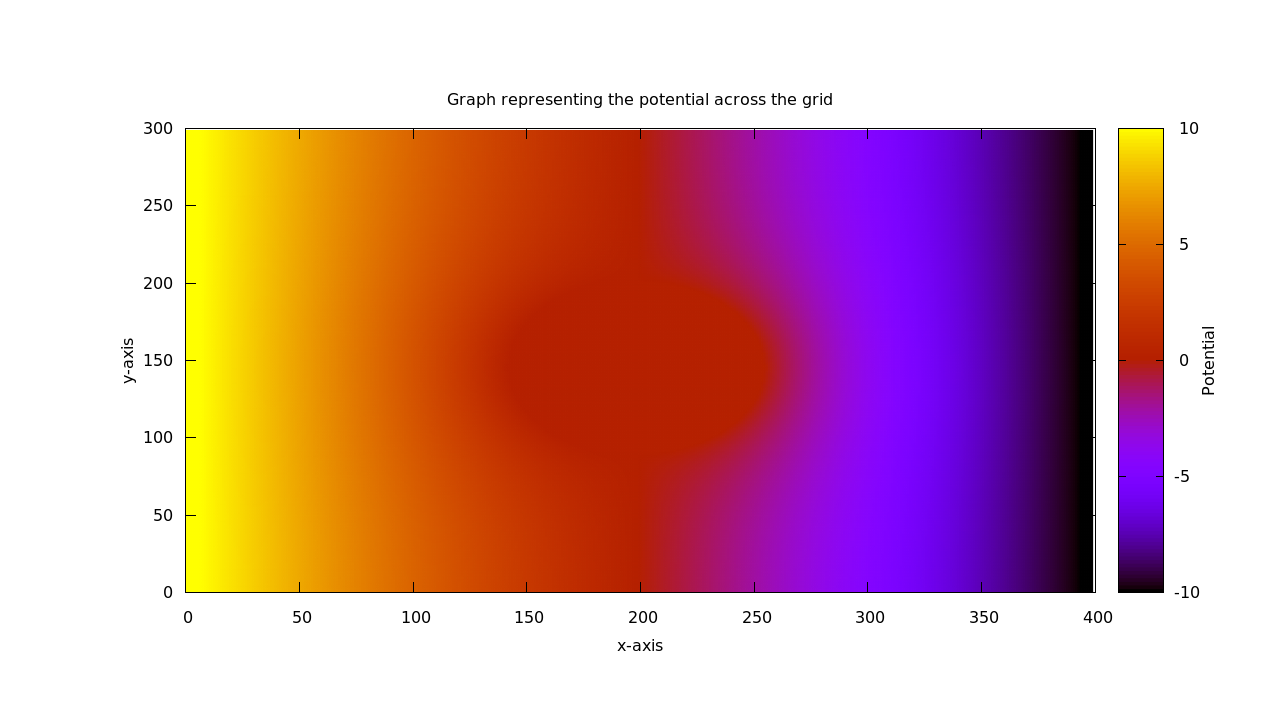
\includegraphics[width=0.95\textwidth, trim = 40mm 20mm 20mm 30mm, clip]{example_potential_plot.png}} % change trim as required to eliminate unnecessary whitespace. trim: left bottom right top
\label{fig:potentialplot}
\caption{A plot representing the electric potential ${\phi}$ at points in the grid.}
\end{figure}

Another output file is also produced to allow the plotting of the electric field. The file contains the x- and y-coordinates as well as the $d{\phi}/dx$ and $d{\phi}/dy$ values, which are approximated. For a point $(x,y)$, the gradient along the x-direction is calculated as the average of the change along one step from the left (-x direction) and one step to the right (+x direction), i.e. $d{\phi}/dx_{x,y} = ( value(x-1,y) - value(x+1,y) ) / 2$. Similarly, for the gradient along the y-direction, the gradient is calculated as the average of the change along one step to the +y direction and one step from the -y direction, i.e. $d{\phi}/dy_{x,y} = ( value(x,y-1) - value(x,y+1) ) / 2$. Here the $\phi$ refers to the potential. The values are written to a file in the format shown in table \ref{table:field_data}.
\begin{table}
    \parbox{0.47\linewidth}{
    \centering
    \begin{tabularx}{0.44\textwidth}{ |XXX| }
        \hline
        $x_1$ & $y_1$ & $value_{1,1}$ \\
        $x_1$ & $y_2$ & $value_{1,2}$ \\
        $x_1$ & $y_3$ & $value_{1,3}$ \\
        & & \\
        $x_2$ & $y_1$ & $value_{2,1}$ \\
        $x_2$ & $y_2$ & $value_{2,2}$ \\
        $x_2$ & $y_3$ & $value_{2,3}$ \\
        & & \\
        $x_3$ & $y_1$ & $value_{3,1}$ \\
        $x_3$ & $y_2$ & $value_{3,2}$ \\
        $x_3$ & $y_3$ & $value_{3,3}$ \\
        \hline
    \end{tabularx}
    \caption{Structure of a file containing information about the potential across the grid. This example is for a 3x3 grid.}
    \label{table:potential_data}
    }
    \hfill
    \parbox{0.47\linewidth}{
    \centering
    \begin{tabularx}{0.44\textwidth}{ |XXXX| }
        \hline
        $x_1$ & $y_1$ & $d{\phi}/dx_{1,1}$ & $d{\phi}/dy_{1,1}$ \\
        $x_1$ & $y_2$ & $d{\phi}/dx_{1,2}$ & $d{\phi}/dy_{1,2}$ \\
        $x_1$ & $y_3$ & $d{\phi}/dx_{1,3}$ & $d{\phi}/dy_{1,3}$ \\
        & & & \\
        $x_2$ & $y_1$ & $d{\phi}/dx_{2,1}$ & $d{\phi}/dy_{2,1}$ \\
        $x_2$ & $y_2$ & $d{\phi}/dx_{2,2}$ & $d{\phi}/dy_{2,2}$ \\
        $x_2$ & $y_3$ & $d{\phi}/dx_{2,3}$ & $d{\phi}/dy_{2,3}$ \\
        & & & \\
        $x_3$ & $y_1$ & $d{\phi}/dx_{3,1}$ & $d{\phi}/dy_{3,1}$ \\
        $x_3$ & $y_2$ & $d{\phi}/dx_{3,2}$ & $d{\phi}/dy_{3,2}$ \\
        $x_3$ & $y_3$ & $d{\phi}/dx_{3,3}$ & $d{\phi}/dy_{3,3}$ \\
        \hline
    \end{tabularx}
    \label{table:field_data}
    \caption{Structure of a file containing information about the electric field across the grid. This example is for a 3x3 grid.}
    }
\end{table}

Again, empty lines are inserted before a change in x-values to make operating gnuplot easier. The data can then be plotted as a vector field in, for example, gnuplot. By setting some functions in gnuplot, one can make the vectors in the field of uniform size (to improve readability) and indicate the magnitude of the vector by colour. An example of such a plot can be seen in figure \ref{fig:vectorfieldplot}.

\begin{figure}[h!]
    \centering
    \setlength\fboxsep{0pt}
    \setlength\fboxrule{0.5pt}
    \fbox{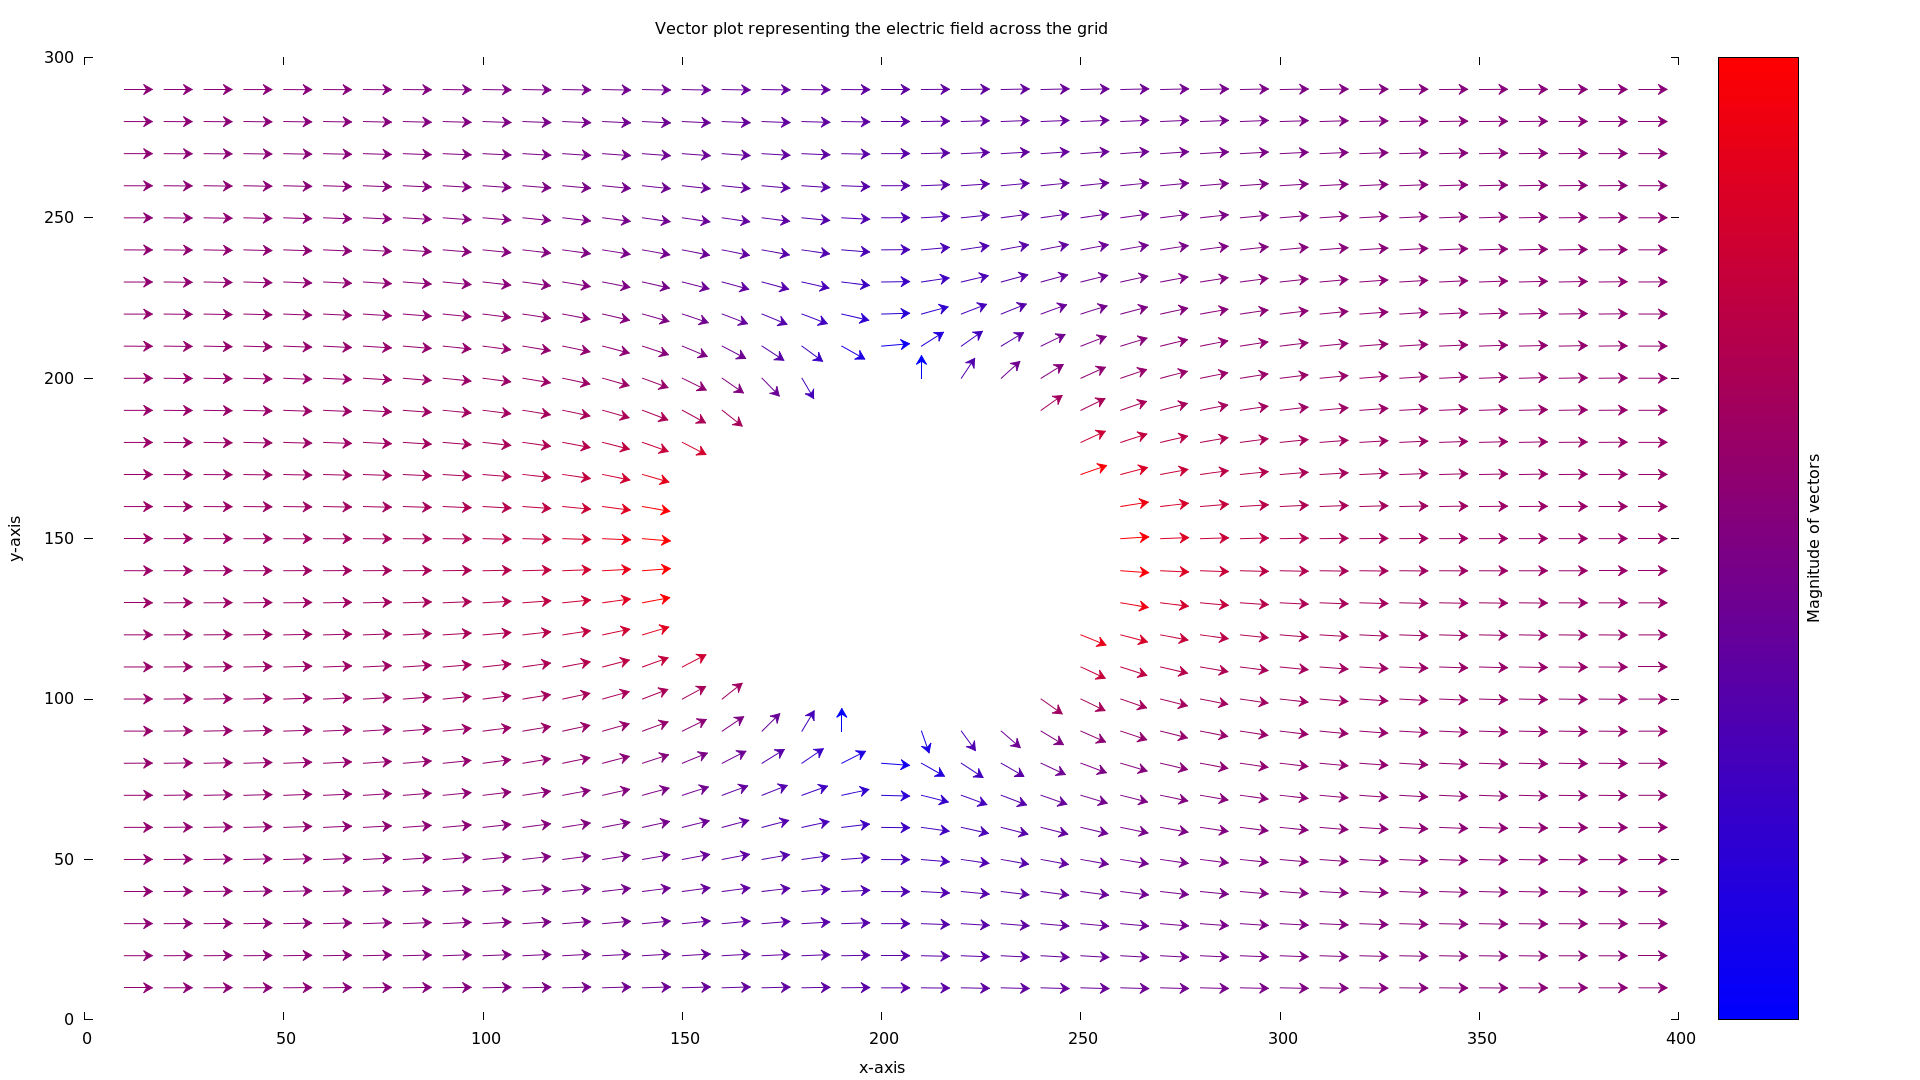
\includegraphics[width=0.95\textwidth, trim = 0mm 0mm 0mm 0mm, clip]{example_vector_field_plot.png}} % trim options: left bottom right top, change to appropriate values if some other image is used and it has too much whitespace around it.
    \caption{A plot representing the electric field calculated for System A, shown as a vector plot with the colour of the vectors indicating the magnitude of the vector: red means large, blue means small.}
    \label{fig:vectorfieldplot}
\end{figure}
 
An equipotential plot is also produced. This uses the same data file as the heatmap-styled plot. The equipotential lines are drawn by the contour function in gnuplot. An example of an equipotential line plot overlaid on a vector field can be seen in figure \ref{fig:vectors_and_contours}.

\begin{figure}[h!]
    \centering
    \setlength\fboxsep{0pt}
    \setlength\fboxrule{0.5pt}
    \fbox{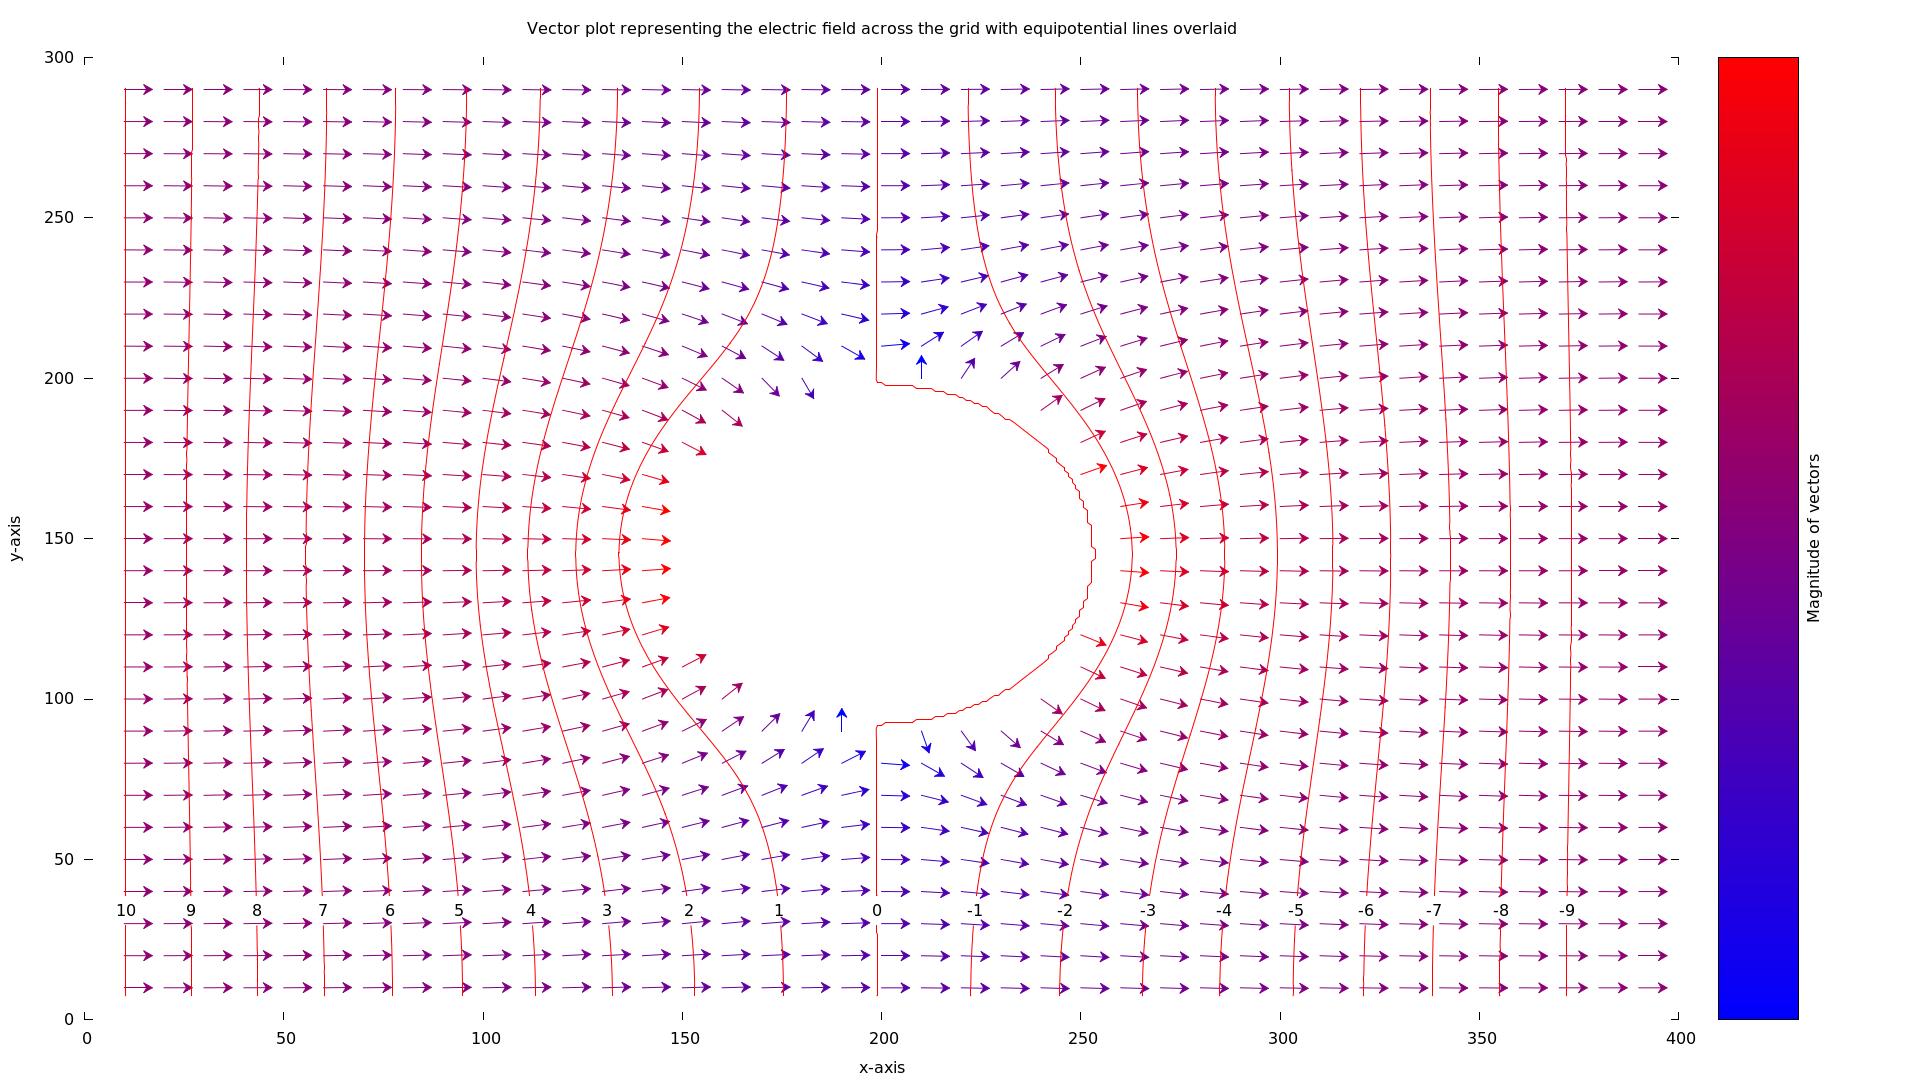
\includegraphics[width=0.95\textwidth, trim = 0mm 0mm 0mm 0mm, clip]{example_vectors_and_contours.png}} % trim options: left bottom right top, change to appropriate values if some other image is used and it has too much whitespace around it.
    \caption{A plot displaying the electric field represented as vectors with equipotential lines overlaid on top of them.}
    \label{fig:vectors_and_contours}
\end{figure}

All of the plotting in the program is done internally via C++ functions which call gnuplot to be run. The source code can be found in the appendix \ref{code:plot.cpp}.

\end{document}

\section{Results}
%The following subsections describe the impact of the different parameters the \lstinline|eStatics| package accepts on the computational performance. The impact can be measured several ways, for example by the time the program takes to finish computing or the number of iterations that were required to reach a certain level of accuracy. 

The \lstinline|eStatics| package accepts the following parameters:
\begin{itemize}
	\item The bitmap representing the system being computed
	\item The potential corresponding to each colour in the bitmap
	\item The maximum iterations the program is allowed to run for
	\item The relaxation level
	\item The desired convergence level
\end{itemize}

Most of the data used for the following graphs was gathered from computations done on System A, if not stated otherwise.

\subsubsection{Iterations}
The number of iterations the program is allowed to run for obviously has a great impact on the length of the computation, unless an accepted convergence level is reached before it. The number of iterations allowed also affects the accuracy of the final approximation, for if the program doesn't reach a predefined convergence level, it will continue converging in on the solution. 

Figure \ref{fig:iterations_vs_accuracy_abs} shows the accuracy of the final approximation compared to the number of iterations the program was run for. The accuracy converges to an absolute error of about $0.5$ per point compared to the analytic solution.

\begin{figure}[h!]
\centering
\setlength\fboxsep{0pt}
\setlength\fboxrule{0.5pt}
\fbox{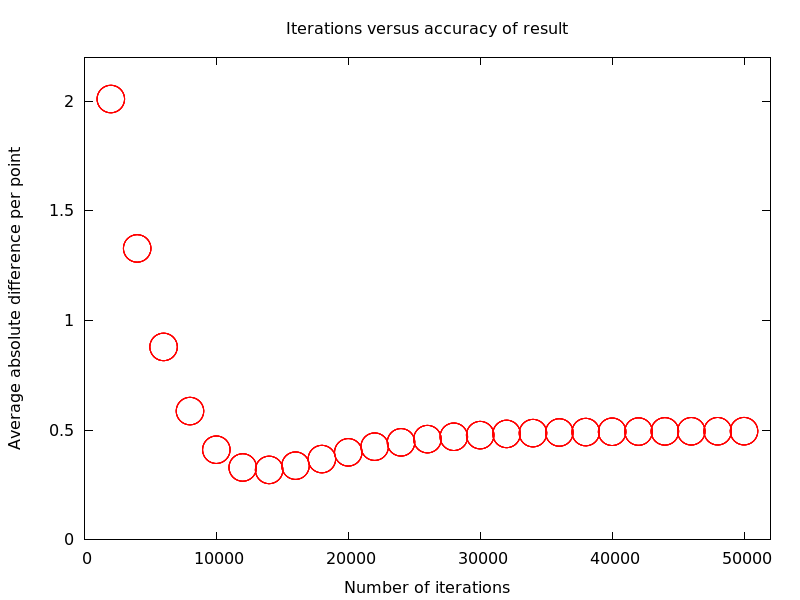
\includegraphics[width=0.95\textwidth, trim = 0mm 0mm 0mm 0mm, clip]{images/iterations_vs_accuracy_abs.png}} % change trim as required to eliminate unnecessary whitespace. trim: left bottom right top
\label{fig:iterations_vs_accuracy}
\caption{Figure showing the average absolute error per point for a given number of iterations calculated.}
\end{figure}

\subsubsection{Convergence}
The predefined convergence level affects the accuracy of the final solution greatly. Most of the error in the computation comes from around the boundaries or edges defined in the bitmap images. A very low desired convergence level is going to require more iterations by the program to reach it, while a high desired convergence may require next to no iterations at all. 

A typical desired convergence level would be somewhere between $10^{-6}$ and $10^{-9}$. This means that successive computations of the same point need to differ by less than $10^{-6}$ to $10^{-9}$ in order for the point to be locked and deemed to have converged at the solution. Setting a lower desired convergence level thus leads to a more precise solution. 

As can be seen on figure \ref{fig:convergence_accuracy}, the numerical approximation converges to an average absolute error of $0.496570$ per point as the level of desired convergence decreases. The $~0.5$ error per point is mostly due to systematic errors from around the boundaries as those are not changed by the numerical method. 

\begin{figure}[h!]
\centering
\setlength\fboxsep{0pt}
\setlength\fboxrule{0.5pt}
\fbox{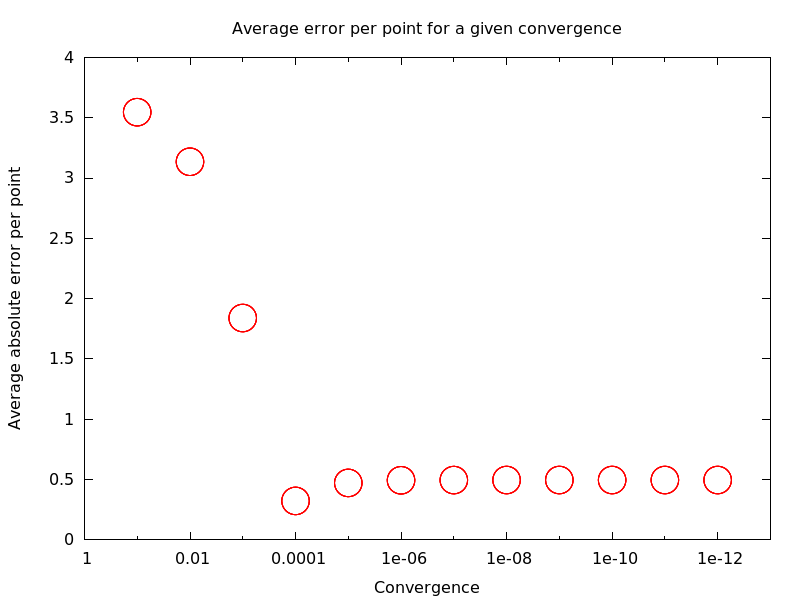
\includegraphics[width=0.95\textwidth, trim = 0mm 0mm 0mm 0mm, clip]{images/convergence_accuracy.png}} % change trim as required to eliminate unnecessary whitespace. trim: left bottom right top
\label{fig:convergence_accuracy}
\caption{Figure showing the average absolute error per point for a given desired convergence.}
\end{figure}

\subsubsection{Relaxation level}
There exists an optimal relaxation level for each system. By plotting the required iterations for different relaxation levels between $1.9$ and $2.0$, as in figure \ref{fig:relax_narrow}, the optimal value is determined to be about $1.9775$, which reduces the number of required iterations to reach a convergence level of $10^{-6}$ from over $42000$ to just $670$, a difference of nearly two orders of magnitude. 

\begin{figure}[h!]
\centering
\setlength\fboxsep{0pt}
\setlength\fboxrule{0.5pt}
\fbox{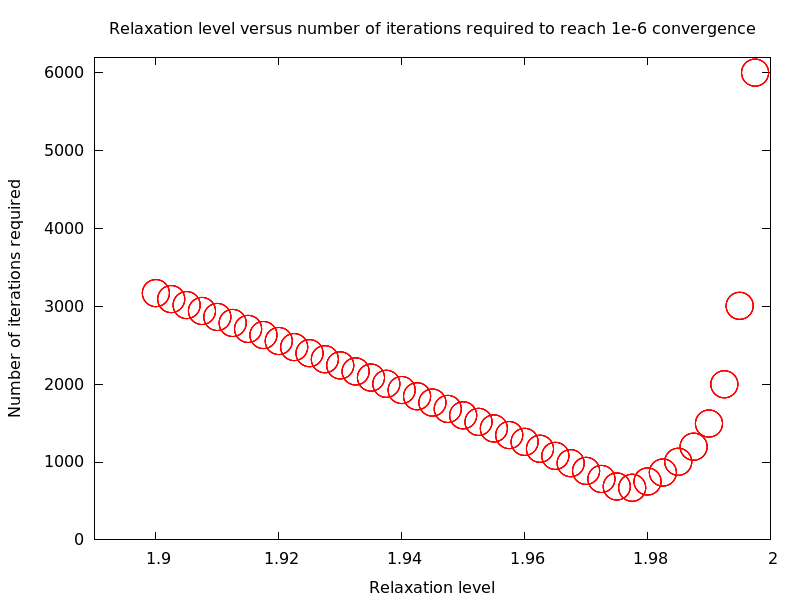
\includegraphics[width=0.95\textwidth, trim = 0mm 0mm 0mm 0mm, clip]{images/relaxation_vs_iterations_narrow.png}} % change trim as required to eliminate unnecessary whitespace. trim: left bottom right top
\label{fig:relax_narrow}
\caption{Figure showing how the number of iterations required to solve System A changes as the relaxation level approaches the optimal value.}
\end{figure}

The accuracy of the solution is not affected negatively by the reduced number of iterations, as the average absolute difference per point is $0.496569$, almost precisely the same as what the solution tends to as the desired convergence tends to zero.

For system C, the optimal relaxation level was determined to be $1.9850$, as can be seen in figures \ref{fig:sysC_relax_wide} and \ref{fig:sysC_relax_narrow}. The program required only $973$ iterations to reach a convergence level of $10^{-6}$ with relaxation level $1.9850$, while with relaxation level of $1.0$, it took over $99000$ iterations. Again, the improvement is nearly two orders of magnitude.

\begin{figure}[h!]
\centering
\setlength\fboxsep{0pt}
\setlength\fboxrule{0.5pt}
\fbox{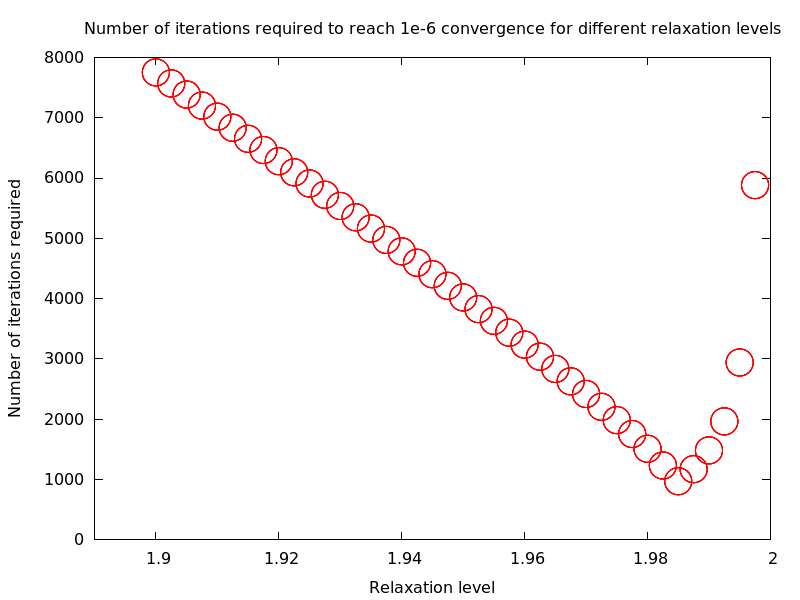
\includegraphics[width=0.95\textwidth, trim = 0mm 0mm 0mm 0mm, clip]{images/sysC_relax_narrow.png}} % change trim as required to eliminate unnecessary whitespace. trim: left bottom right top
\label{fig:sysC_relax_narrow}
\caption{Figure showing how the number of iterations required to solve System C changes as the relaxation level approaches the optimal value.}
\end{figure}

\subsubsection{Multithreading}
Multithreading can have a great impact on the time taken to run a program. Figure \ref{fig:multiple_multithreads} shows the impact on computation time when using different number of threads on \lstinline|eStatics|. The difference becomes more and more substantial when each thread has more work to do, so the multithreading process is ideal for computing larger grids.

\begin{figure}[h!]
\centering
\setlength\fboxsep{0pt}
\setlength\fboxrule{0.5pt}
\fbox{\includegraphics[width=0.95\textwidth, trim = 0mm 0mm 0mm 0mm, clip]{images/multiple_multithreads.png}} % change trim as required to eliminate unnecessary whitespace. trim: left bottom right top
\label{fig:multiple_multithreads}
\caption{Comparing the time required for a varying number of iterations with 1-8 threads.}
\end{figure}


\section{Conclusion}
In conclusion, the Laplace equation was presented and derived in the context of
electromagnetism. Its general analytical solution in plane polar co-ordinates was
deduced, as well as a particular analytical solution for the case of a grounded
cylinder between two charged planes.

Finite difference methods were introduced and their necessity discussed, and the
Laplace equation was discretised. Five different examples of relaxation methods were
presented and compared, \emph{vis-\`{a}-vis} their relative error and convergence, and
the optimal method was shown to be Checkerboard updating with successive over-relaxation.

A software package, \lstinline|eStatics|, capable of solving Laplace's equation for
arbitrary constant boundary conditions, was described, and example output of the
package for different boundary conditions were shown.

Several improvements could have been made to the software: adaptive step-sizing could
have been implemented in regions of quickly changing potential; the software could be
made able to solve systems with more than four different potentials; and constant boundary
conditions that vary with position could have been examined. The software could be
generalised to be able to solve Laplace's equation given only von Neumann boundary
conditions, where the normal component of the gradient of the potential is specified
at each boundary. 

Further work is proposed in the use of alternative numerical methods in the
numerical approximations of Laplace's equation, namely fast Fourier transforms,
multigrid methods and nine-point stenciling. Additionally, the numerical approximations
to the solutions of Poisson's equation could be studied.

%include BibTex bibliography
\bibliography{main}

%start of appendix
\appendix
\section{Appendices}

\subsection{Method Comparison}
\label{app:compare}
Figure~\ref{fig:compare} show the numerical approximation for the potential for each
method.


Figure~\ref{fig:stats} show the statistics for each method.

\begin{figure}
\centering 
\begin{subfigure}{0.8\textwidth}
	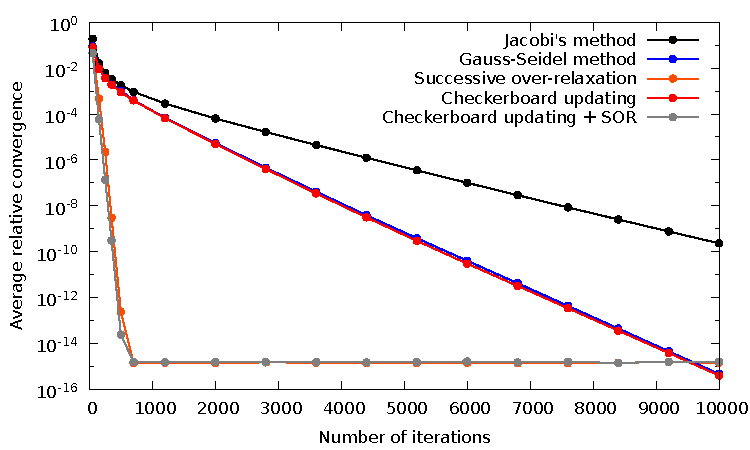
\includegraphics[scale=0.8]{rel_convergence.pdf}
	\caption{Average relative convergence, between successive approximations for the potential of each method, versus number of iterations}
	\label{fig:conv}
\end{subfigure}

\begin{subfigure}{0.8\textwidth}
	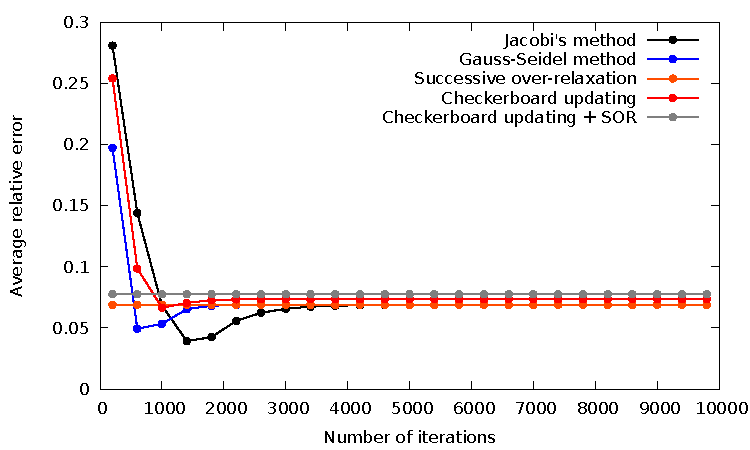
\includegraphics[scale=0.8]{rel_error.pdf}
	\caption{Average relative error of each method, as compared to the analytical solution, versus number of iterations}
	\label{fig:err}
\end{subfigure}

\begin{subfigure}{0.8\textwidth}
	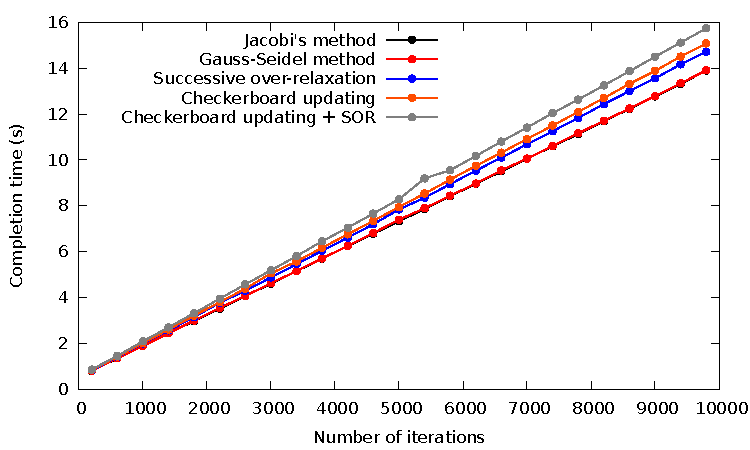
\includegraphics[scale=0.8]{time.pdf}
	\caption{CPU time taken by each method versus number of iterations}
	\label{fig:time}
\end{subfigure}
\caption{Summary of the method comparison statistics}
\label{fig:stats}
\end{figure}

\subsection{Algorithm for Software Package}

\begin{algorithm}
\begin{algorithmic}[1]
\Procedure{The Jacobi iterative method}{}
\State declare variables:
\State $V \gets$ potential on plates
\State $\delta \gets$ position step-size
\State $d \gets$ distance between plates
\State $h \gets$ height of plates
\State $r \gets$ radius of cylinder
\State $its \gets$ number of iterations
\State $nx \gets \frac{d}{\delta}$ 
\State $ny \gets \frac{h}{\delta}$ 
\State specify boundary potentials:
\For {$j=1$ to $ny$}
   \State $u_{j, 1} = +V$
   \State $u_{j, nx} = -V$
\EndFor
\For {$k=1$ to $nx$}
   \State $u_{1, k} \gets V-\frac{2Vj}{nx}$
   \State $u_{ny, k} \gets V-\frac{2Vj}{nx}$
\EndFor
\State find solution:
\For {$i=1$ to $its$}
   \For {$j=2$ to $ny-1$}
      \For {$k=2$ to $nx-1$}
         \If {$(j \delta-\frac{1}{2} d)^2+(k \delta-\frac{1}{2} h)^2<r^2$}
            \State $u_{j, k} \gets 0$
         \Else
            \State $u_{j,k} \gets \frac{1}{4}(u_{j-1,k}+u_{j+1,k}+u_{j,k-1}+u_{j,k+1})$
         \EndIf
      \EndFor
   \EndFor
\EndFor
\State find electric field:
\For {$j=1$ to $ny-1$}
   \For {$k=1$ to $nx-1$}
      \State $(Ex)_{j, k} \gets -\left(u_{j,k+1}-u_{j,k-1}\right)/2\delta$
      \State $(Ey)_{j,k} \gets -\left(u_{j+1,1}-u_{j-1,k}\right)/2\delta$
   \EndFor
\EndFor
\State plot potential and field
\EndProcedure
\end{algorithmic}
\end{algorithm}

\subsection{Flowchart for System}
\label{app:flowchart}
\begin{figure}[htbp!]
\begin{center}
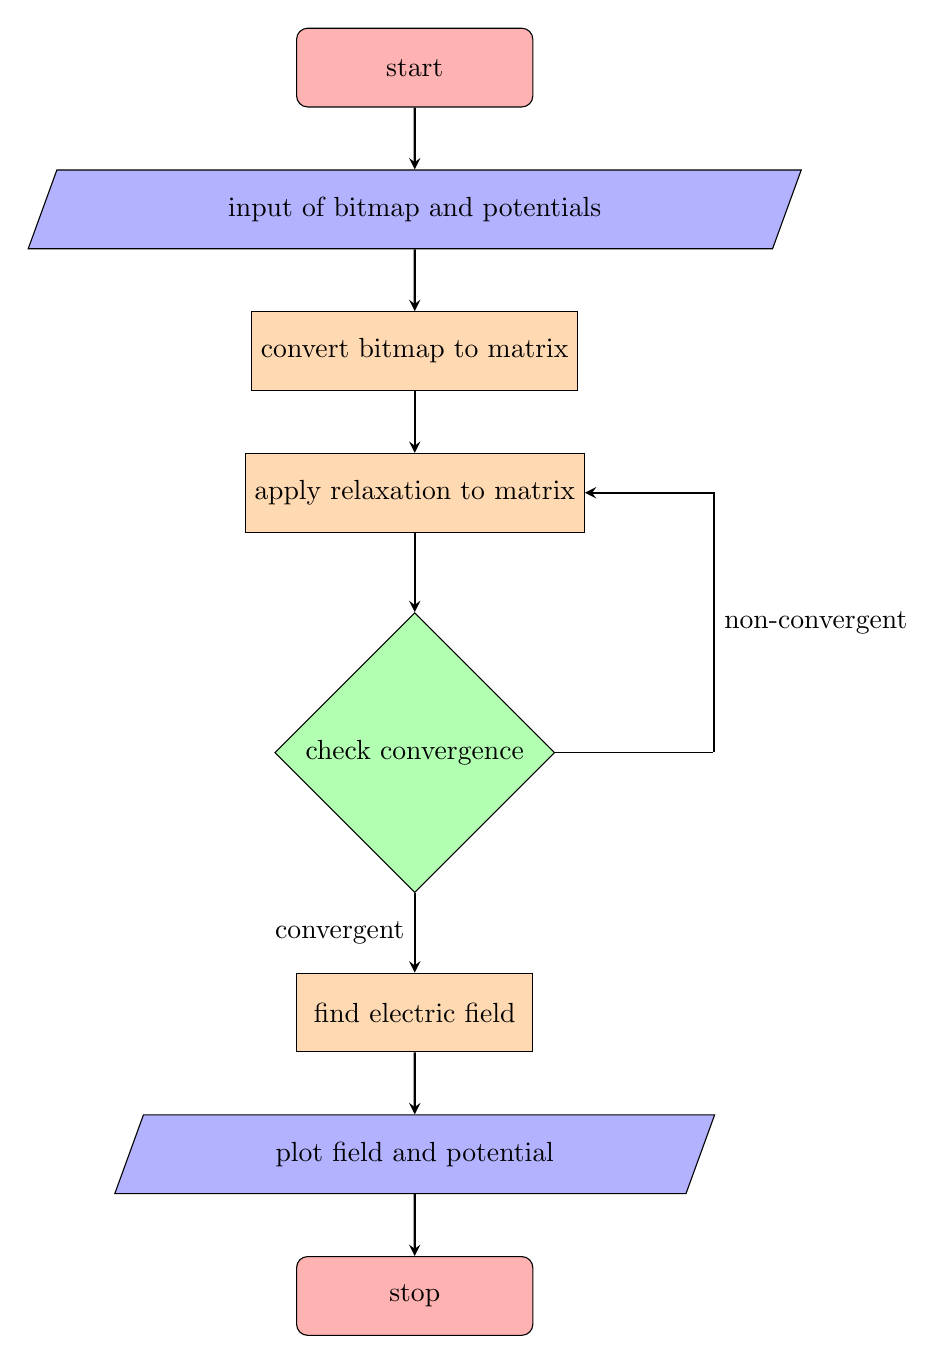
\begin{tikzpicture}[node distance=1.8cm]

\node (start) [startstop] {start};
\node (in1) [io, below of=start] {input of bitmap and potentials};
\node (pro1) [process, below of=in1] {convert bitmap to matrix};
\node (pro2) [process, below of=pro1] {apply relaxation to matrix};
\node (dec1) [decision, below of=pro2, yshift=-1.5cm] {check convergence};
\node (inv) [inner sep=0, minimum size=0, right of=dec1, xshift=2cm] {}; % invisible node
\node (pro3) [process, below of=dec1, yshift=-1.5cm] {find electric field};
\node (out1) [io, below of=pro3] {plot field and potential};
\node (stop) [startstop, below of=out1] {stop};

\draw [arrow] (start) -- (in1);
\draw [arrow] (in1) -- (pro1);
\draw [arrow] (pro1) -- (pro2);
\draw [arrow] (pro2) -- (dec1);
\draw [arrow] (dec1) -- node[left] {convergent} (pro3);
\draw (dec1) -- (inv);
\draw [arrow] (inv) |- node[pos=0.25, right] {non-convergent} (pro2);
\draw [arrow] (pro3) -- (out1);
\draw [arrow] (out1) -- (stop);

\end{tikzpicture}
\end{center}
\caption{Flowchart of steps in software package}
\label{fig:flowchart}
\end{figure}

\end{document}
